% !TEX root = ../main.tex

% standrd model is not capitalized is not a proper noun
\chapter{The Higgs boson and CP violation in the Standard Model and beyond}

The discovery of the Higgs boson in 2012 \cite{Aad:2012tfa,Chatrchyan:2012xdj} has been one of the greatest successes of the standard model (SM) of elementary particles, that is currently the most broadly accepted theory describing the fundamental constituents of matter and 
their interactions among each other. Although having defied unnumerous tests, it is insufficient because it cannot explain approved experimental observations such as the matter-antimatter asymmetry in the observable universe. 
Moreover, only three of the four known fundamental forces - the electromagnetic, strong, weak and gravitational force - can be described as a quantum theory. 
Currently, no verified quantum theory of gravitation exists and the SM and general relativity form two complementary descriptions of nature.
There are theories which solve these problems by introducing new physics that goes beyond the description of the SM. In general physicists follow two approaches to search for physics beyond the standard model (BSM). These are direct searches for  new particles and phenomena and indirect searches, where 
BSM physics leads to inconsistencies between measured SM parameters. Consequently, new physics would have been detected if any deviation from the prediction of the SM was observed in a precision measurement. 
Since the discovery of the Higgs boson, a major scientific effort has been performed to measure all the particles' properties. These include measurements of the mass $m_\text{H}$ \cite{combined_mass_Higgs}, the decay width $\Gamma_\text{H}$\,\cite{atlas_Higgswidth}, the spin and parity quantum numbers \cite{Run1_spin_parity,Run1_spinparity_ATLAS}. So far no deviation from the SM predition has been found. 
The precise determination of the properties of the Higgs boson under parity and charge-conjugation transformations, namely the CP properties, is, however, still a major challenge in Higgs physics. Being predicted as a scalar $J^\text{PC}=0^{++}$ particle, 
observations up to now only exclude the pure pseudoscalar scenario. A small pseudoscalar admixture to the prediction of the SM is still a valid scenario. The detection of such an admixture would prove CP violation in the Higgs sector, contributing potentially to the matter-antimatter asymmetry in the universe. This thesis presents a framework for an analysis that is dedicated to the precise
measurement of the CP properties of the Higgs boson in the gluon-gluon fusion process.
Beginning with a brief summary about the current understanding of elementary particles with the focus on the properties of the Higgs boson, a theoretical framework for performing a measurement of CP properties in fermionic couplings 
of the Higgs boson using an effective field theory (EFT) is motivated. In chapter \ref{chap:cms} an overview about the CMS Detector and the LHC at CERN and the reconstruction of particles from recorded signals is given.
Chapter \ref{chap:analysis} presents the setup, statistical tools, and quotes the result in terms of an expected sensitivity for the measurement of the CP mixing angle of the Higgs boson to top quarks.

\section{The Standard Model}
The SM describes the constituents of matter by \textit{elementary particles} and the fundamental \textit{electromagnetic, weak and strong forces}. 
Each particle is considered to be an excitation of a field with certain properties under symmetry transformations. Interactions between particles are based on the principle of \textit{local gauge invariance} leading to bosons that mediate these interactions. 
The SM is mathematically formulated in the framework of relativistic quantum field theories (QFT) and is expressed through a Lagrange density $\Lagr_\text{SM}$ that is invariant under local gauge transformations of the form $\text{SU(3)}_\text{C} \times \text{SU(2)}_\text{L} \times \text{U(1)}_\text{Y}$. 
The corresponding gauge bosons are 8 gluons with color charge resulting from the $\text{SU(3)}_\text{C}$, three weak bosons with weak isospin from $\text{SU(2)}_\text{L}$ and  one boson with hypercharge from $\text{U(1)}_\text{Y}$.
The importance of local gauge invariance can be inferred from t'Hooft's proof \cite{tHooft:1972tcz} that every locally gauge invariant QFT is renormizable. Renormizability enables the prevention of divergencies originating from energy ranges that lie beyond the scope of the theory by restricting the energy scale to the scale of the problem.
Feynman diagrams, which are a graphical representation of  perturbational calculus, are used to derive the matrix element that encapsulates all necessary information to calculate physics observables such as cross sections, angular distributions and decay rates.

\begin{figure}[h!]
    \centering
    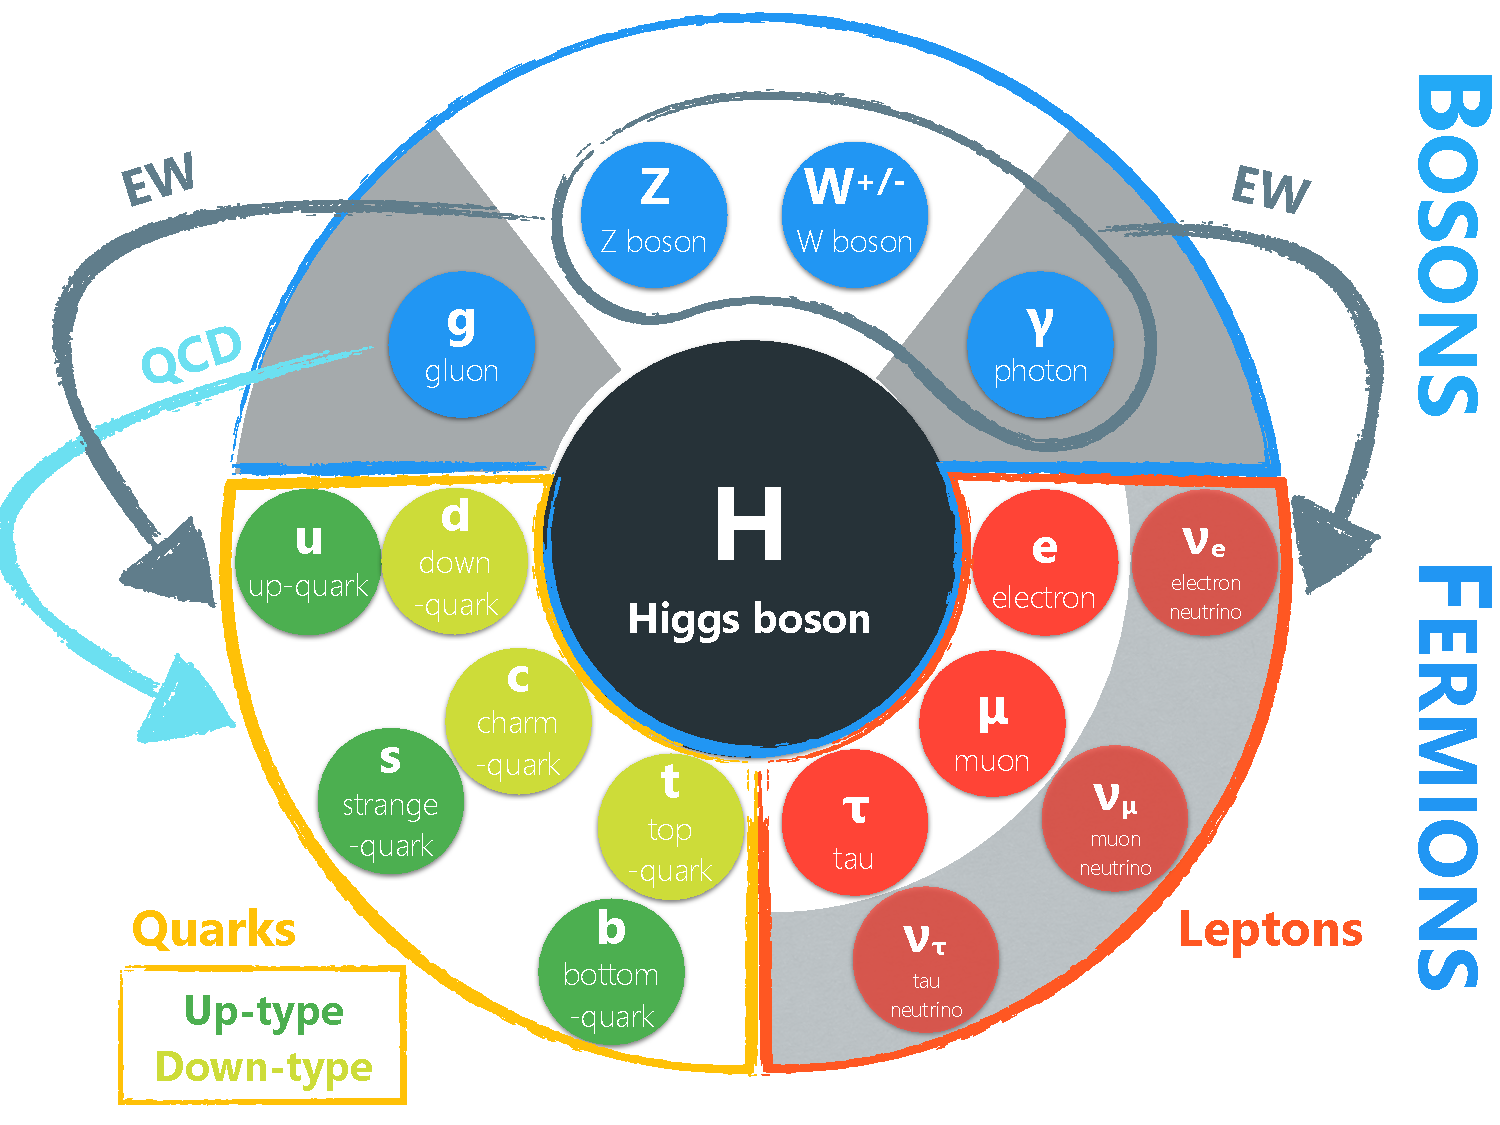
\includegraphics[width=.7\textwidth]{Figures/theory/Masterthesis_diagrams_SM/Masterthesis_diagrams_SM.pdf}
    \caption[Particle content and description of the interactions of the SM.]{Particle content and description of the interactions of the SM. Fermions can be categorized into quarks and leptons. 
    According to their similar quantum numbers, but very different masses, both types of fermions are further divided into three generations that come as left-handed doublets and right-handed singlets.
    The four gauge bosons are the mediators of the strong, electromagnetic and weak interactions. By means of electroweak symmetry breaking (EWSB), the Higgs boson gives rise to the masses of the weak bosons and all fermions except for the neutrinos, that are 
    massless particles within the description of the SM and do also not form right-handed singlets. The arrows indicate that an interaction can take place between the associated bosons
     and fermions (EW: Electroweak interaction, QCD: Strong interaction). The shaded area behind some of the particle indicates that they do not couple directly to the Higgs boson and are as a consequence massless.}\label{theory:SM_infographics}
\end{figure}

\subsection{Elementary particles and interactions} 

Elementary particles are entities that do not constitute of more fundamental particles. Each particle posseses distinct quantum numbers such as mass, spin, electric charge, and color charge that precisely define its
properties and possible behaviour regarding the interaction with other particles. 
Based on the spin, it is possible to group all particles into \textit{fermions} with spin-1/2 and \textit{bosons} with integer spin.
The twelve fermions of the SM can be considered as the building blocks of matter. They come up as left-handed doublets and right-handed singlets in so-called generations with increasing mass but otherwise similar physical properties. 
\textit{Quarks} carry color charge and are the only group of elementary particles that interacts via the strong interaction, which is modeled within the theory of quantum chromodynamics (QCD). They also 
have an electric charge of $+\frac{\text{2}}{\text{3}}\text{e}$ or $-\frac{\text{1}}{\text{3}}\text{e}$ for \textit{up-type quarks} and \textit{down-type quarks}, respectively, and carry weak isospin implying that they also take part in the electroweak interaction (EW), which is the unified theory describing the electromagnetic and weak interactions. 
The remaining six fermions are called \textit{leptons}. 
The electron, muon and tau lepton have an electric charge and participate in the EW. The massless and chargeless neutrinos interact only weakly. Although it has been confirmed through the observation of neutrino-oscillations that they must possess very small masses \cite{PhysRevLett.81.1562,Ahmad:2001an,PhysRevLett.89.011301}, neutrinos are considered massless within the SM.
Bosons are force-mediators and responsible for the interaction between fermions. Thereby, the Higgs boson plays an important role as it gives mass to the fermions and EW bosons, as discussed below. \\
The sketch in \figreft{theory:SM_infographics} shows the particle content and the interactions of the SM.

\subsubsection{Quantum Chromodynamics}\label{subsec:QCD}
\begin{figure}[h!]
    \centering
    \begin{tikzpicture}[line width=1.5pt, scale=1]
% \draw[step=0.5cm, very thin, transparent] (0cm,0cm) grid (3cm,2cm);
\draw[fermion] (0cm,1.5cm) -- (1.5cm,0.5cm);
\fill[black] (0.62cm:1.57cm) circle (0.1cm);
\node at (0cm-0.3cm,1.5cm) {\textbf{\textit{q}}};
\draw[fermion] (1.5cm,0.5cm) -- (3cm,1.5cm);
\node at (3cm+0.3cm,1.5cm) {\textbf{\textit{q}}};
\draw[gluon] (1.5cm,0.5cm) -- (1.5cm, -1.2cm);
\node at (1.5cm, -1.3cm) {\textbf{\textit{g}}};
\end{tikzpicture}%
\begin{tikzpicture}[line width=1.5pt, scale=1]
% \draw[step=0.5cm, very thin, transparent] (0cm,0cm) grid (3cm,2cm);
\draw[gluon] (0cm, 1.5cm) -- (0.75cm,0cm);
\node at (-0cm-0.3cm,1.5cm) {\textbf{\textit{g}}};
\fill[black] (0:0.75cm) circle (0.1cm);
\draw[gluon] (0.75 cm,0cm) -- (0cm,-1.5cm);
\node at (0cm-0.3cm,-1.5cm) {\textbf{\textit{g}}};
\draw[gluon] (0.75cm,0cm) -- (2.25cm, 0cm);
\node at (2.25cm+0.3cm, 0cm) {\textbf{\textit{g}}};
\end{tikzpicture}%
\begin{tikzpicture}[line width=1.5pt, scale=1]
% \draw[step=0.5cm, very thin, transparent] (0cm,0cm) grid (3cm,2cm);
\draw[gluon] (0cm,1.5cm) -- (1.5cm,0cm);
\node at (0cm-0.3cm,1.5cm) {\textbf{\textit{g}}};
\draw[gluon] (1.5cm,0cm) -- (3cm,1.5cm);
\node at (3cm+0.3cm,1.5cm) {\textbf{\textit{g}}};
\draw[gluon] (1.5cm,0cm) -- (0cm, -1.5cm);
\node at (3.3cm, -1.5cm) {\textbf{\textit{g}}};
\draw[gluon] (3cm, -1.5cm) -- (1.5cm,0cm);
\node at (0cm-0.3cm, -1.5cm) {\textbf{\textit{g}}};
\fill[black] (0:1.5cm) circle (0.1cm);
\end{tikzpicture}%

    \caption[Standard vertices of QCD.]{Standard vertices of QCD. Gluon coupling to a pair of quarks (left), three gluon-vertex (middle) and 
    four-gluon vertex (right).}\label{theory:QCD_vertices}
\end{figure}

Gluons ($g$) are mediators of the strong force. There are eight gluon generators $T^a$, that are related to the $\text{3\times3}$ Gellmann-matrices $\lambda^a$  for the $\text{SU(3)}_\text{C}$ symmetry group with the relation $T^a = \frac{1}{2}\lambda^a$, corresponding 
to the eight possible non-trivial combinations and superpositions of three different colors $c$ and their associated anti-colors $\bar{c}$. 
As gluons possess an effective color charge $c\bar{c}$, too, they interact with themselves causing the possible standard vertices of QCD depicted in \figreft{theory:QCD_vertices}. The corresponding coupling structure for the QCD vertices in the Feynman diagrams is 
\begin{equation}    
    \propto g_\text{S} \frac{1}{2}\lambda^a_{ij} \gamma^\mu
\end{equation}
with a strong coupling constant $g_\text{S}$ and color factor $\lambda^a_{ij}$, that is the $ij$-th component of the Gellmann matrix of the generator $a \in \left[ 1..8\right]$. \newpage{}
$\gamma^{\mu}$ is the vector of Dirac matrices as it 
appears in the Dirac equation \cite{Thomson:2013zua}.\newline{}
The range of gluon interactions is restricted to the size of the color-neutral hadrons formed by the quarks. This \textit{color confinement} is supported by the experimental observation that
quarks and gluons do not propagate freely and hypothesizes that only particles with a net color charge equal to zero can propagate in free space. 
As a consequence, a quark or gluon being produced in a high-energy physics interaction undergoes the process of \textit{hadronization} and produces a shower of hadrons, called \textit{jet}.


\subsubsection{Quantum Flavourdynamics (QFD)}\label{subsec:QFD}
\begin{figure}[h!]
    \centering
    \begin{tikzpicture}[line width=1.5pt, scale=1]
% \draw[step=0.5cm, very thin, transparent] (0cm,0cm) grid (3cm,2cm);
\draw[fermion] (0cm, 1.5cm) -- (0.75cm,0cm);
\node at (-0cm-0.3cm,1.5cm) {\textbf{\textit{f}}};
\draw[fermion] (0.75 cm,0cm) -- (0cm,-1.5cm);
\node at (0cm-0.3cm,-1.5cm) {\textbf{\textit{f}}};
\draw[vector] (0.75cm,0cm) -- (2.25cm, 0cm);
\node at (2.25cm+0.3cm, 0cm) {\textbf{\textit{$\gamma$}}};
\fill[black] (1:0.75cm) circle (0.1cm);
\end{tikzpicture}%
\begin{tikzpicture}[line width=1.5pt, scale=1]
% \draw[step=0.5cm, very thin, transparent] (0cm,0cm) grid (3cm,2cm);
\draw[fermion] (0cm,1.5cm) -- (1.5cm,0.5cm);
\node at (0cm-0.3cm,1.5cm) {\textbf{\textit{f}}};
\draw[fermion] (1.5cm,0.5cm) -- (3cm,1.5cm);
\node at (3cm+0.3cm,1.5cm) {\textbf{\textit{f}}};
\draw[vector] (1.5cm,0.5cm) -- (1.5cm, -1.2cm);
\node at (1.5cm, -1.5cm) {\textbf{\textit{$\gamma$}}};
\fill[black] (0.62cm:1.57cm) circle (0.1cm);
\end{tikzpicture}%
\begin{tikzpicture}[line width=1.5pt, scale=1]
% \draw[step=0.5cm, very thin, transparent] (0cm,0cm) grid (3cm,2cm);
\draw[fermion] (0cm,1.5cm) -- (1.5cm,0.5cm);
\node at (0cm-0.3cm,1.5cm) {\textbf{\textit{f}}};
\draw[vector] (1.5cm,0.5cm) -- (3cm,1.5cm);
\node at (3cm+0.3cm,1.5cm) {\textbf{\textit{$\gamma$}}};
\draw[fermion] (1.5cm,0.5cm) -- (1.5cm, -1.2cm);
\node at (1.5cm, -1.5cm) {\textbf{\textit{f}}};
\fill[black] (1.5cm,.55cm) circle (0.1cm);
\end{tikzpicture}%

    \caption[Standard vertices of QED.]{The three standard vertices of QED describe the annihilation of a fermion-antifermion pair into a photon (s-channel, left), 
    the scattering of a fermion by exchange of a photon (t-channel, middle) and the emission of a photon (right).}\label{theory:QED_vertices}
\end{figure}
The photon (\gamma) is the mediator of the electromagnetic force and couples to all particles that have an electric charge $Q$. 
Quantum electrodynamics (QED) introduces the photon field $A$ that produces the vertices indicated in \figreft{theory:QED_vertices}. The structure
for the fermion current in the Feynman diagrams at an interaction vertex of QED for fermions described by the Dirac spinor $u$ and the Dirac matrices is
\begin{equation}
    \propto Q \bar{u}\gamma^\mu u.  
\end{equation}
The $W^{\pm}$ bosons are responsible for the flavour-changing charged current (FCCC) of the weak interaction and couple to all left-handed particles possessing weak isospin $T_\text{3}$. 
The charged current produces vertices of the form
\begin{equation}
    \propto g_\text{W}\frac{1}{2}\gamma^\mu \li 1-\gamma^5\re,
\end{equation}
where $g_\text{W}$ is the weak coupling constant and $\gamma^5 = i\gamma^0\gamma^1\gamma^2\gamma^3$.\newline{}
The weak and the electromagnetic interactions
are unified within the electroweak model of Glashow, Salam and Weinberg (GSW model)\,\cite{Klapdor1989}. The neutral current (NC) induced by the Z boson is evoked by the third neutral generator $W_3^0$ of the $\text{SU(2)}_\text{L}$ gauge group to the weak isospin $T^\text{(3)}_\text{W}$ through 
mixing with a photon-like neutral field $B$ that obeyes a further $\text{U(1)}_\text{Y}$ gauge group to the weak hypercharge $Y$. Moreover, during the mixing the QED photon field $A$ is retrieved naturally. The hypercharge
is connected to both electric charge $Q$ and weak isospin $T$ by the relation
\begin{equation}
    Y = 2 \li Q - T_\text{W}^{\li 3 \re} \re. 
\end{equation}
The Feynman diagrams of the production of a W and a Z boson are shown in \figreft{theory:QFD_vertices}.
\begin{figure}[h!]
    \centering
    \begin{tikzpicture}[line width=1.5pt, scale=1]
% \draw[step=0.5cm, very thin, transparent] (0cm,0cm) grid (3cm,2cm);
\draw[fermion] (0cm, 1.5cm) -- (0.75cm,0cm);
\node at (-0cm-0.5cm,1.5cm) {\textbf{\textit{l,q}}};
\draw[fermion] (0.75 cm,0cm) -- (0cm,-1.5cm);
\node at (0cm-0.5cm,-1.5cm) {\textbf{\textit{$\boldsymbol{\nu}_\mathbf{l}$,q$\prime$}}};
\draw[vector] (0.75cm,0cm) -- (2.25cm, 0cm);
\node at (2.25cm+0.3cm, 0cm) {\textbf{\textit{W}}};
\fill[black] (0:.75cm) circle (0.1cm);
\end{tikzpicture}%
\begin{tikzpicture}[line width=1.5pt, scale=1]
% \draw[step=0.5cm, very thin, transparent] (0cm,0cm) grid (3cm,2cm);
\draw[fermion] (0cm, 1.5cm) -- (0.75cm,0cm);
\node at (-0cm-0.6cm,1.5cm) {\textbf{\textit{l,$\boldsymbol{\nu}_\mathbf{l}$,q}}};
\draw[fermion] (0.75 cm,0cm) -- (0cm,-1.5cm);
\node at (0cm-0.6cm,-1.5cm) {\textbf{\textit{l,$\boldsymbol{\nu}_\mathbf{l}$,q}}};
\draw[vector] (0.75cm,0cm) -- (2.25cm, 0cm);
\node at (2.25cm+0.3cm, 0cm) {\textbf{\textit{Z}}};
\fill[black] (0:.75cm) circle (0.1cm);
\end{tikzpicture}%

    \caption[Weak boson production Feynman graphs.]{The standard vertices of QFD describe the production of a W boson by FCCC and the production of a Z boson. There are also t-channel diagrams which are not shown here. 
            The fermions participating in the production of the W boson must possess left-handed helicity eigenvalues. }\label{theory:QFD_vertices}
\end{figure}

\subsection{The Higgs mechanism}

The Higgs mechanism is an integral part of the SM, because it ensures the self-consistency of the theory. Bosons that are introduced
through a gauge symmetry are necessarily massless particles, because mass terms of the form $m^2V^{\mu\nu}V_{\mu\nu}$ as they appear in the Klein-Gordon equation break the previously required local gauge invariance. 
Opposed to that claim, it was observed that the weak gauge bosons have very large masses, which are
responsible for the short-rangeness of the weak interaction \cite{ARNISON1983103}. The Higgs mechanism proposed independently by Brout, Englert and Higgs et al. in 1964 \cite{PhysRevLett.13.508,PhysRevLett.13.321,PhysRevLett.13.585,1964PhL....12..132H,PhysRev.145.1156} applies the 
principle of \textit{spontaneous symmetry breaking} to a scalar field with a potential of the form given in \figreft{theory:Higgs_potential}. \newline{}
\begin{figure}[!h]
    \centering
    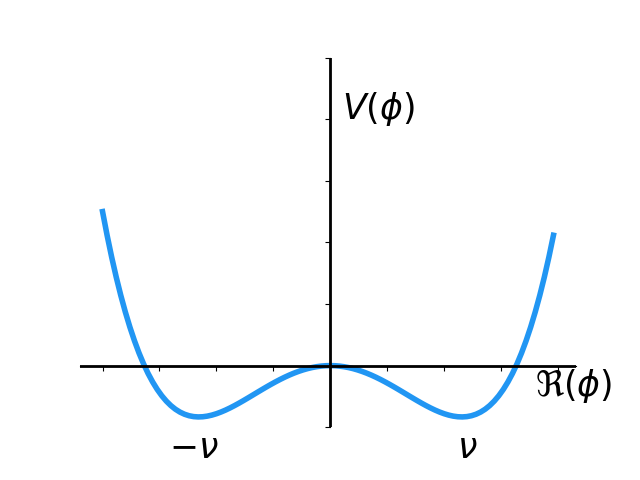
\includegraphics[width = .5\textwidth]{Figures/theory/Higgs_potential}
    \caption[Higgs field potential.]{Projection onto the real plane of the Higgs field potential. The positions of the minima are degenerate and have a value that is different from zero. Thus, the non-zero vacuum expectation value $\nu = \text{246\,{GeV}}$ breaks 
    the symmetry of the Higgs field .}\label{theory:Higgs_potential}
\end{figure}%
In the SM two complex scalar fields are placed within a doublet of the weak isospin
\begin{equation}
    \phi = \tdvec{\phi^+}{\phi^0}. 
\end{equation}
This gives rise to four degrees of freedom that create the masses of the two W bosons and the Z boson through interaction with the scalar field. The fourth degree belongs to the 
massive boson corresponding to the scalar field. This boson is called \textit{Higgs boson}. 
Without loss of generality the scalar field can be chosen to be a real constant by gauge fixing. In the unitary gauge the ground state is
\begin{equation}
    \bra{0}\phi\ket{0} = \tdvec{0}{\nu} 
\end{equation}
with a real, positive constant $\nu$.
The Higgs mechanism creates terms of the form 
\begin{equation}
    \frac{1}{8}\nu^2 g_\text{W}^2 \li W^{\li 1 \re}_\mu W^{\li 1 \re, \mu} + W^{\li 2 \re, \mu} W^{\li 2 \re}_\mu \re + \frac{1}{8} \nu^2 \li g_\text{W} W^{\li 3 \re\,  \mu} - g^\prime B^\mu \re \li g_\text{W} W^{\li 3 \re}_\mu - g^\prime B_\mu \re 
\end{equation}
in the Lagrangian. They have the form of mass terms, and therefore the masses of the weak gauge bosons can be read off or rather be derived within the GSW model to be
\begin{equation}
    m_\text{W} = \frac{1}{2}g_\text{W}\nu \tab \text{and} \tab  m_\text{Z} = \frac{1}{2}\nu \sqrt{g_\text{W}^2 +g^{\prime2}}.
\end{equation}   
This implies that by measuring the masses and coupling constants of the W bosons and the Z boson $m_\text{W/Z}$ and $g_\text{W}/g^\prime$ the vacuum expectation value can be calculated
\begin{equation} 
    \nu = \text{246\,{GeV}}.
\end{equation} 

\subsubsection{Higgs boson Yukawa couplings}
The SM Higgs mechanism generates the masses of the W and Z bosons and solves the mass term problem for them. The 
different behaviour of left-handed and right-handed fermions, $\bar{f}_\text{L}$ and $f_\text{R}$,  under $\text{SU(2)}_\text{L}$ transformation produces Dirac mass terms of the form 
form
\begin{equation}
    \Lagr_\text{f} = -m\bar{f}f  = -m \li \bar{f}_\text{L}f_\text{R} + \bar{f}_\text{R}f_\text{L}\re
\end{equation} 
that break the gauge symmetry again.
Nevertheless, it can be shown that terms of the form 
\begin{equation}
    -y_\text{f} \left[ \bar{L}\phi R + \bar{R}\phi^\dagger L \right]
\end{equation}
and equivalent terms with the complex conjugate Higgs doublet
\begin{equation}
     \phi_\text{C} = \tdvec{-\nu-H}{0}
\end{equation}
of the form
\begin{equation}
    -y_\text{f} \left[ \bar{L}\phi_\text{C} R + \bar{R}\phi_\text{C}^\dagger L \right]
\end{equation}
 are invariant under transformations of the complete $\text{SU(2)}_\text{L} \times \text{U(1)}_\text{Y}$ symmetry group. 
Thereby, $L$ and $R$ denote the left-handed fermion doublet and right-handed fermion singlet, respectively.
For this reason, it is possible to retrieve expressions that have the form of Dirac mass terms 
\begin{equation}
    \Lagr_{\text{mass}} \propto -y_\text{f} \nu \li \bar{f}_\text{L} f_\text{R} + \bar{f}_\text{R} f_\text{L} \re = -y_\text{f} \nu  \bar{f}f.
\end{equation} 
The Yukawa coupling constants $y_\text{f}$, that were introduced above, are not predicted by the SM Higgs mechanism and must be measured. 
This means, $y_\text{f}$ is proportional to the fermion mass by construction
\begin{equation}
    y_\text{f} = \frac{m_\text{f}}{\nu}.
\end{equation}
Moreover, interaction terms between the fermions and the Higgs boson appear that are proportional to the Yukawa couplings
\begin{equation}
    \Lagr_\text{Y} \propto  -y_\text{f} H \li \bar{f}_\text{L} f_\text{R} + \bar{f}_\text{R} f_\text{L} \re = -y_\text{f} \bar{f}fH.
\end{equation} 

\subsubsection{Properties of the Higgs boson}

% describe the production and the decay
% show the relevant Feynman graphs
% pinn down the necessary cross sections
%
Given the mass of the Higgs boson of $\text{125.18\,GeV}$ \cite{Patrignani:2016xqp} the coupling strengths to other particles are fixed within the SM and production cross sections in proton-proton collisions and branching ratios can be predicted.
The two most important production processes are shown in \figreft{theory:feynman_production}.\newline{}
\begin{figure}[h!]
    \centering
    \begin{subfigure}{.49\textwidth}
        \centering
        \begin{tikzpicture}[line width=1.5pt, scale=1.2]
% \draw[step=0.5cm, very thin, transparent] (0cm,0cm) grid (4cm,2cm);

\draw[gluon] (0cm,1.25cm) -- (1.25cm,1.25cm);
\node at (0cm-0.3cm,1.25cm) {$g$};

\draw[gluon] (0cm,-1.25cm) -- (1.25cm,-1.25cm);
\node at (0cm-0.3cm,-1.25cm) {$g$};

\draw[fermion] (1.25cm,1.25cm) -- (1.25cm,-1.25cm);
\draw[fermion] (1.25cm,1.25cm) -- (2.25cm,0cm);
\draw[fermion] (2.25cm,0cm) -- (1.25cm,-1.25cm);
\node at (1.25cm-0.3cm,0cm) {$t$};
\node at (2cm-0.3cm,1.2cm) {$t$};
\node at (2cm-0.3cm,-0.2cm) {$\bar{t}$};
\draw[scalar, ctcoloraccessory] (2.25cm,0cm) -- (3.5cm,0cm);
\node at (3cm-0.3cm,-.3cm) {$H$};
\fill[black] (1.25cm,1.3cm) circle (0.1cm);
\fill[black] (0:2.25cm) circle (0.1cm);
\fill[black] (1.25cm,-1.3cm) circle (0.1cm);
\end{tikzpicture}
 
        \caption{\,Higgs boson produced via ggF.}\label{theory:feynman_production:ggF}
    \end{subfigure}
    \begin{subfigure}{.49\textwidth}
        \centering
        \begin{tikzpicture}[line width=1.5pt, scale=1]
% \draw[step=0.5cm, very thin, transparent] (0cm,0cm) grid (4cm,2cm);

\draw[fermion] (0cm,1.25cm) -- (1.25cm,1.25cm);
\node at (0cm-0.3cm,1.25cm) {$q$};
\draw[fermion] (1.25cm,1.25cm) -- (3cm,1.5cm);
\node at (3cm+0.3cm,1.5cm) {$q$};

\draw[fermion] (0cm,-1.25cm) -- (1.25cm,-1.25cm);
\node at (0cm-0.3cm,-1.25cm) {$q'$};
\draw[fermion] (1.25cm,-1.25cm) -- (3cm,-1.5cm);
\node at (3cm+0.3cm,-1.5cm) {$q'$};

\draw[vector] (1.25cm,1.25cm) -- (1.5cm,0cm);
\draw[vector] (1.25cm,-1.25cm) -- (1.5cm,0cm);

\draw[scalar, ctcoloraccessory] (1.5cm,0cm) -- (3cm,0cm);
\node at (2.5cm-0.3cm,-.3cm) {$H$};

\node at (1.5cm+0.3cm,.75cm) {$V$};
\node at (1.5cm+0.3cm,-.75cm) {$V$};
\fill[black] (1.25cm,1.25cm) circle (0.1cm);
\fill[black] (1.25cm,-1.25cm) circle (0.1cm);
\fill[black] (0:1.5cm) circle (0.1cm);
\end{tikzpicture}
 
        \caption{\,Higgs boson produced via VBF.}\label{theory:feynman_production:VBF}
\end{subfigure}
    \caption[Higgs boson production processes.]{Feynman graphs of the two most efficient production processes of the Higgs boson.}\label{theory:feynman_production}
\end{figure}
At the LHC \textref{sec:LHC} the most efficient production mechanism is the gluon-gluon fusion process (\textit{ggF}) \fref{theory:feynman_production:ggF}. The LHC is a proton collider which means the energy of the actual collision
is determined by the amount of momentum that the two colliding partons (gluon or quark) carry inside the proton. The momentum is a fraction $x$ of the total proton momentum $p_{\,\text{P}}$ and defined by the parton density functions that depict the probability that a parton carries a 
momentum fraction $x$ \cite{PhysRev.179.1547}. At the LHC energies the parton density function for gluons peaks at low values of $x$. These $x$ values are matching to the production of a Higgs boson at 125\,GeV mass.
Together with the Higgs coupling to the top quark which is in the order $\origo{1}$, this leads to the relatively high cross section of $\mathsf{\sigma_{gg\rightarrow H}} = \text{43.92\,pb}$ \cite{Heinemeyer:2013tqa}
for the ggF production process. Later in this thesis, ggF events with two initial-state jets are selected to study the CP properties of the Higgs boson \figref{theory:ggH2j_feynman}. 
These events are a next-to-next-to-leading-order (NNLO) QCD contributions and result, thus, in a cross section that is suppressed by a factor of $g_\text{s}^2$. Nevertheless, the NNLO ggF process contributes with a cross section of $\mathsf{\sigma_{gg\rightarrow Hjj}} = \text{3.98\,{pb}}$, which is still a bit larger than
the contribution from vector boson fusion (VBF)  with a cross section of $\mathsf{\sigma_{VV\rightarrow H}} = \text{3.748\,pb}$. As VBF is characterized by two forward jets originating from the remnants of the two quarks that radiate off the
vector bosons producing the Higgs boson, the topology of VBF is very similar to that of ggF events in association with two jets.

The Higgs production is decoupled from the decay because no spin information is transferred through a scalar or pseudoscalar resonance. For this reason, Higgs boson production processes can be studied with any possible decay mode. The branching ratios 
of the most frequent decay modes are given in \tabreft{theory:higgs:decay}. 

The decay into a pair of tau leptons $H\rightarrow \tau^+\tau^-$ is used to identify Higgs bosons in this thesis as this analysis built upon the SM search for the Higgs boson decaying into tau leptons \cite{Sirunyan:2017khh}. This provides on the 
one hand a relatively high yield of Higgs bosons \tabref{theory:higgs:decay} and on the other hand a settled framework for the selection of Higgs bosons. 
In the following the $H\rightarrow \tau^+\tau^-$ decay is abbreviated by $H\rightarrow \tau\tau$ keeping in mind that the tau leptons in the final state have electric charges. 

\begin{table}[!]
    \centering
    \caption[Higgs boson decay mode branching ratios.]{Decay modes and branching ratios (BR) of the SM Higgs boson \cite{Patrignani:2016xqp}.}\label{theory:higgs:decay}
    \begin{tabular}{lll}
    \toprule
    Decay mode                  & BR / \% & Remark                                                                                \\ \hline
    $H\rightarrow b\bar{b}$     & 57.8                    & Highest branching fraction, but large QCD background \cite{hbb}.                                  \\
    $H\rightarrow WW^*$         & 21.6                    & Off-shell produced W-boson \cite{ATLAS:2014aga}.                     \\
    $H\rightarrow gg$           & 8.6                     & Not detectable at LHC.                                                                \\
    \multirow{2}{*}{$H\rightarrow \tau^+\tau^-$ } & \multirow{2}{*}{6.4}                     & Largest direct coupling to leptons. \\
                            &                                         & Relatively low background compared to $b\bar{b}$ \cite{Sirunyan:2017khh}. \\
    $H\rightarrow c\bar{c}$     & 2.9                     & Not discovered yet, very large QCD backgrounds.                                        \\
    \multirow{2}{*}{$H\rightarrow ZZ^*$  }       & \multirow{2}{*}{2.7}                     & Utilized for Higgs boson discovery.                                           \\
                                            &                         & Very low background in $ZZ\rightarrow 4l$ \cite{Aad:2012tfa,Chatrchyan:2012xdj}.   \\
    \multirow{2}{*}{$H\rightarrow \gamma\gamma$} & \multirow{2}{*}{0.2}                     & Utilized for Higgs boson discovery.  \\
                                            &                         & Clear signature and low backgrounds \cite{Aad:2012tfa,Chatrchyan:2012xdj}.    \\  \bottomrule                                                  
    \end{tabular}
\end{table}

\section{CP violation}
Investigating the behaviour of physics processes under symmetry transformations can provide fundamental information about the nature of the interaction.
For example, physical processes are studied regarding the situation that 
\begin{ct_version_list}
    \item the direction of time is inverted or
    \item the coordinate system is spatially inverted.
\end{ct_version_list}
Invariance under these transformations gives fundamental insight into the physics of the process, because according to 
Emmy Noethers' theorem any symmetry leads to a conserved quantity \cite{zbMATH02611626,zbMATH02611883}.
This section gives an overview about how elementary particle interactions behave under 
parity, charge-conjugation and time-reversel transformations and the implications of violations from these laws.
\newpage{}
\subsection{Symmetry transformations}
The SM is based on the CPT-theorem, that implies that every QFT is invariant under the combination of 
\begin{ct_version_list}
    \item parity transformation $\mathcal{P}$, that inverts the coordinate system with the transformation $\vec{r}\rightarrow -\vec{r}$,
    \item charge-conjugation $\mathcal{C}$, that inverts the sign of every additive quantum number of the particle, thus turning a particle into an anti-particle and vice-versa, and 
    \item time-reversel $\mathcal{T}$, that inverts the sign of the time component $t\rightarrow -t$ and consequently changes the direction of time \cite{CPT_lueders,Pauli1988}. 
\end{ct_version_list}
The interaction terms appearing in the Lagrangian are lorentz-invariant bilinear forms that provide a distinct behaviour under these transformations. An overview about 
the different structures and their properties is given in \tabreft{theory:bilinears}.

\begin{table}[h]
    \centering
    \caption[Bilinear transformation properties.]{Behaviour of bilinear forms under $\mathcal{P}$, $\mathcal{C}$ and $\mathcal{T}$  transformations. The proofs are summarized in Ref. \cite{Nason11}. Here, $\li -1 \re^\mu$ denotes that the transformation is $+1$ if $\mu=0$ and $-1$ for $\mu \in \left[ 1,2,3\right]$, where $\mu$ is the 
     $\mu$-th component of the four-vector.}\label{theory:bilinears}
    \begin{tabular}{lcccc}
        \toprule
        Type         & Form                                 & $\mathcal{P}$               & $\mathcal{C}$ & $\mathcal{T}$                \\ \midrule
        Scalar       & $\bar{\psi}\phi$                     & $+1$                   & $+1$     & $+1$                   \\
        Pseudoscalar & $\bar{\psi}\gamma^5\phi$             & $-1$                   & $+1$     & $-1$                   \\
        Vector       & $\bar{\psi}\gamma^\mu \phi$          & $\li -1 \re^{\mu}$    & $-1$     & $\li -1 \re^{\mu}$ \\
        Axial vector & $\bar{\psi}\gamma^\mu \gamma^5 \phi$ & $-\li -1 \re^{\mu}$     & $+1$     & $\li -1 \re^{\mu}$ \\
        Tensor       & $\bar{\psi}\sigma^{\mu\nu} \phi$     & $\li -1 \re^{\mu}\li -1 \re^{\nu}$   & $-1$     &  $ -\li -1 \re^{\mu}\li -1 \re^{\nu}$ \\ \bottomrule
    \end{tabular}
\end{table}

From \tabreft{theory:bilinears} it can be inferred that 
\begin{ct_version_list}
    \item QED and QCD are invariant under CP-transformations because their fermion currents are vector couplings as given in sections \ref{subsec:QCD} and \ref{subsec:QFD}.
    \item The charged current interaction maximally violates both parity and charge-conjugation transformations individually as experimentally proven by \cite{PhysRev.105.1413}. Mathematically, the coupling structure of the weak interaction of the form $\bar{f}\gamma^\mu-\gamma^\mu \gamma^5 f$ explains this.
            The consequence of this violation is that there are no couplings to right-handed neutrinos and left-handed anti-neutrinos in the SM \cite{PhysRev.109.1015}.
\end{ct_version_list}    

Any quantum state that is eigenstate of the corresponding transformation has the eigenvalue $\pm 1$. For the CP transformation this implies, for instance,
\begin{equation}
    \mathcal{CP}\ket{\psi^{\pm}_\text{CP}} = \pm \ket{\psi^{\pm}_\text{CP}},
\end{equation} 
where +1 and -1 are the eigenvalues of the CP-even and CP-odd eigenstates, respectively. Any superposition of CP-even and CP-odd states is no longer an eigenstate of the CP transformation (see eq. \eqref{eq:CP}). Thus, CP violation is observed:
\begin{equation}\label{eq:CP}
    \mathcal{CP}\ket{\psi_\text{CP}} = \mathcal{CP}\li a \cdot \ket{\psi^{+}_\text{CP}} + b \ket{\psi^{-}_\text{CP}}  \re =  a \cdot \ket{\psi^{+}_\text{CP}} -  b \ket{\psi^{-}_\text{CP}} \neq \pm \ket{\psi_\text{CP}}.
\end{equation} 

\subsection{CP violation in the Standard Model}

Summarizing the properties of the weak interaction under C and P transformations above, one would expect that the weak interaction 
is at least invariant under simultaneous C and P transformations. In contrast to that, evidence for CP violation was reported in 
neutral Kaon decays and mixing  \cite{Christenson:1964fg,Bluemer:503743,Gorini:884851} and in B meson systems \cite{PhysRevLett.87.091801,Aubert:2002ya,PhysRevD.68.051101,PhysRevLett.91.201802,PhysRevLett.89.281802}.
Recently, the T2K experiment reported indications that CP conservation is also not conform with the neutrino sector \cite{Abe:2017uxa} pointing towards CP violation also there. CP violation in the SM has its source in the complex phase of the 3x3 CKM-matrix which relates the mass eigenstates of the quarks to their
weak eigenstates that couple to the weak gauge bosons \cite{PhysRev.105.1413}. 
CP violation occurs because this complex phase is irreducible and appears, thus, in the matrix elements for box diagrams in mixing processes, for example. 
For a brief overview about the occurence of CP violation in the SM the reader is pointed to Ref. \cite{Thomson:2013zua}. A complete and detailed theoretical description, even beyond the SM, is given in Ref. \cite{Branco:1999fs}.

\subsubsection{CP violation and the early universe}

According to the big bang theory, matter and antimatter must have been produced in equal amounts initially. 
This implies that all matter should have been annihilated into gamma rays when the density, and consequently the interaction rate, was still high enough 
in the early universe. Obviously some matter survived the annihilation phase, leading to the formation of stars and galaxies. Measurements
strongly indicate that no major abundances of antimatter are present in the observable universe today. Quantitatively, this can be 
inferred from the matter-antimatter asymmetry $\eta_\text{Asymmetry}$ that is defined by the difference of baryon $n_\text{B}$ and antibaryon $n_{\bar{\text{B}}}$ densities in relation to the cosmic microwave background photon density
\begin{equation}
    \eta_\text{Asymmetry} = \frac{n_\text{B} - n_{\bar{\text{B}}}}{n_{\gamma}} \sim 10^{-9}.
\end{equation}
In principle, the SM provides the theoretical framework required by the Sakharov conditions\,\cite{Sakharov:1967dj} that describe a physical configuration leading to a 
matter-antimatter asymmetry:
\begin{ct_version_list}
    \item Baryon number violation,
    \item CP violation and
    \item a deviation from thermal equilibrium.
\end{ct_version_list}
An estimate for the total amount of CP violation in the SM can be derived using the Jarlskog determinant $\mathcal{J}$ as defined in Ref. \cite{PhysRevLett.55.1039}. 
A dimensionless quantity can be constructed by dividing  the temperature present at the condensation of the Higgs field, when the masses of the quarks were generated, at a temperature $T_\text{EWSB}=\text{125\,{GeV}}$
\begin{equation}
    A_\text{CP} = \frac{\mathcal{J}}{T_\text{EWSB}^{12}} \approx 10^{-19} << \eta \sim 10^{-9}.
\end{equation}
\newpage{}
Comparing this roughly estimated value to the observed baryon asymmetry, it can be seen that the CP nonconservation in the SM is not large enough to explain the Baryogenesis. Therefore, the search for potentially larger sources of CP violation beyond the SM is strongly encouraged.

\subsection{Effective field Lagrangian}

In this analysis an approach utilizing an effective field theory (EFT) is followed. Thereby, the SM Lagrangian $\Lagr_\text{SM}$ 
is modified with kinematically possible new terms. Often processes are introduced at a cut-off scale $\Lambda$. Models relevant for studies aiming to determine the 
spin and parity ($J^\text{PC}$) properties of the Higgs boson are constructed by taking the SM Lagrangian, excluding the Higgs boson, and adding new terms associated with a boson $H$ with model-specific $J^\text{PC}$ properties. 
An EFT provides some advantages compared to other types of BSM theory types, that are, for instance, that
\begin{ct_version_list}
    \item only a limited set of new parameters and combinations of parameters needs to be introduced and studied,
    \item the SM is naturally recovered at low energies,
    \item every EFT is fully renormizable since orders of $\sqrt{s}/\Lambda$ in the expansion become small,
    \item if necessary, the model may be extended by adding  higher order effects or by introducing further interactions and particles.
\end{ct_version_list}
As described in Ref. \cite{Artoisenet2013} such a Lagrangian for a 
spin-0 boson has the form
\begin{equation}
    \Lagr_{\text{eff}} = \Lagr_{\text{SM Higgs}} + \Lagr_{H\text{(J=0)}}. 
\end{equation}%
For the analysis in this thesis a Lagrangian $\Lagr_{H\text{(J=0)}}$ is used that 
\begin{ct_version_list}
    \item allows for a mixing between scalar and pseudoscalar couplings of the boson,
    \item is limited to three-point interactiosn between $H$, fermions and vector bosons, meaning that only \textit{Hff} and \textit{HVV} vertices are considered, and
    \item assumes that the resonance at 125\,{GeV} belongs to a single boson. 
\end{ct_version_list} 

\subsubsection{Determining the Higgs Yukawa coupling to the top quark}
The CP properties of the Higgs boson can be fully deduced from its couplings in the production and its decay because it is a scalar or a pseudoscalar particle. There are studies dedicated 
to the measurement of the CP properties in couplings to vector bosons \cite{CMS-AN-17-034} and to tau leptons in the tau
decay channel \cite{claudia_thesis}. This analysis is dedicated to measure the CP properties in fermionic couplings in the production process which means that 
the Yukawa coupling to quarks needs to be investigated. 
At the LHC Higgs bosons are predominantly produced via ggF. As gluons are massless particles they do not couple directly to the Higgs boson. An intermediate quark loop 
is needed, and thus the effective coupling to gluons in the ggF process is studied to examine the Yukawa couplings of the Higgs boson. 
In principle, any quark flavour can run in the loop between the gluons and the Higgs boson but due to the large coupling of the top quark to the Higgs boson it becomes the 
dominant contribution. In Ref. \cite{DelDuca:2001eu} it was shown that the heavy-top quark limit $m_\text{t}\rightarrow \infty$, where the top quark is much heavier than the Higgs boson, 
is a very good approximation for these studies. Therefore, this simplification is considered within this analysis implying that the Yukawa coupling to the 
top quark is directly inferred from the effective \textit{ggH} coupling.
Compared to the VBF production process which occurs via the t-channel, there are no visible remnants that can be used to deduce the coupling parameters. 
Therefore, two initial-state partons need to be radiated off as indicated in the Feynman graphs in figure \ref{theory:ggH2j_feynman}. These
appear as two jets in the detector. Consequently, the signature of the ggF events, that is used to study the fermionic couplings of the Higgs boson, is very similar to the typical VBF Higgs production topology with its two forward jets. 
For this reason, the $\mathsf{qq\rightarrow{H}}$ process is considered as a background in this analysis.

\begin{figure}[h]
    \centering
    \begin{tikzpicture}[line width=1.5pt, scale=1]
% \draw[step=0.5cm, very thin, transparent] (0cm,0cm) grid (3.5cm,2cm);

\draw[fermion] (-0.75cm,1.5cm) -- (0cm,1.5cm);
\draw[fermion] (0cm,1.5cm) -- (3cm,1.5cm);

\draw[fermion] (-0.75cm,-1.5cm) -- (0cm,-1.5cm);
\draw[fermion] (0cm,-1.5cm) -- (3cm,-1.5cm);

\draw[gluon]  (1.25cm,1cm) -- (0cm,1.5cm);
\node at (0.75cm-0.3cm,.9cm) {\textbf{\textit{g}}};

\draw[gluon] (0cm,-1.5cm) -- (1.25cm,-1cm);
\node at (0.75cm-0.3cm,-0.9cm) {\textbf{\textit{g}}};

\draw[fermion] (1.25cm,1cm) -- (1.25cm,-1cm);
\draw[fermion] (1.25cm,1cm) -- (2.25cm,0cm);
\draw[fermion] (2.25cm,0cm) -- (1.25cm,-1cm);
\node at (1.25cm+0.3cm,0cm) {\textbf{\textit{t}}};
\draw[scalar, ctcoloraccessory] (2.25cm,0cm) -- (3cm,0cm);
\node at (3cm-0.3cm,-.3cm) {\textbf{\textit{H}}};
\fill[black] (0:2.25cm) circle (0.1cm);
\fill[black] (1.25cm,1cm) circle (0.1cm);
\fill[black] (1.25cm,-1cm) circle (0.1cm);
\fill[black] (0cm,-1.5cm) circle (0.1cm);
\fill[black] (0cm,1.5cm) circle (0.1cm);
\end{tikzpicture}

    \begin{tikzpicture}[line width=1.5pt, scale=1.2]
% \draw[step=0.5cm, very thin, transparent] (0cm,0cm) grid (3.5cm,2cm);

\draw[gluon] (-1.25cm,1.0cm) -- (-0.5cm,1.0cm);
\draw[fermion] (-0.5cm,1.0cm) -- (1cm,1.0cm);
\draw[gluon] (1cm,1.cm) -- (2cm,1.cm);

\draw[fermion] (-1.25cm,-1.5cm) -- (-0.5cm,-1.5cm);
\draw[fermion] (-0.5cm,-1.5cm) -- (2cm,-1.5cm);


\draw[gluon] (-0.5cm,-1.5cm) -- (-.5cm,-.5cm);
\draw[fermion] (-0.5cm,-.5cm) -- (-.5cm,1.0cm);
\draw[fermion] (1cm,1.0cm) -- (1cm,-.5cm);
\draw[fermion] (1cm,-.5cm) -- (-0.5cm,-.5cm);

\draw[scalar, ctcoloraccessory] (1cm,-0.5cm) -- (2cm,-0.5cm);
\node at (1.8cm-0.3cm,-.8cm) {\textbf{\textit{H}}};
\fill[black] (-0.5cm,1.0cm) circle (0.1cm);
\fill[black] (1.0cm,1.0cm) circle (0.1cm);
\fill[black] (1.0cm,-0.5cm) circle (0.1cm);
\fill[black] (-0.5cm,-0.5cm) circle (0.1cm);
\fill[black] (-0.5cm,-1.5cm) circle (0.1cm);
\end{tikzpicture}

    \begin{tikzpicture}[line width=1.5pt, scale=1]
% \draw[step=0.5cm,  very thin, transparent] (0cm,0cm) grid (3.5cm,2cm);


\draw[gluon] (-1cm,1cm) -- (0.cm,1cm);
\node at (-1cm-0.3cm,1cm) {\textbf{\textit{g}}};

\draw[gluon] (-1cm,-1cm) -- (0.cm,-1cm);
\node at (-1cm-0.3cm,-1cm) {\textbf{\textit{g}}};

\draw[gluon] (1.5cm,1.5cm) -- (3.cm,1.5cm);
\node at (3cm+0.3cm,1.5cm) {\textbf{\textit{g}}};

\draw[gluon] (1.5cm,-1.5cm) -- (3.cm,-1.5cm);
\node at (3cm+0.3cm,-1.5cm) {\textbf{\textit{g}}};

\draw[fermion] (0cm,-1cm) -- (0cm,1cm);
\draw[fermion] (0cm,1cm) -- (1.5cm,1.5cm); 
\draw[fermion] (1.5cm,1.5cm) -- (2.25cm,0cm);
\draw[fermion] (2.25cm,0cm) -- (1.5cm,-1.5cm);
\draw[fermion] (1.5cm,-1.5cm) -- (0cm,-1cm);

\draw[scalar, ctcoloraccessory] (2.25cm,0cm) -- (3cm,0cm);
\node at (3cm-0.3cm,-.3cm) {\textbf{\textit{H}}};
\fill[black] (0:2.25cm) circle (0.1cm);
\fill[black] (0cm,1cm) circle (0.1cm);
\fill[black] (0cm,-1cm) circle (0.1cm);
\fill[black] (1.5cm,1.5cm) circle (0.1cm);
\fill[black] (1.5cm,-1.5cm) circle (0.1cm);
\end{tikzpicture}

    \caption[ggF plus two jets diagrams.]{Feynman graphs for the production of a Higgs boson via ggF in association with two initial state radiation partons $\mathsf{gg\rightarrow H+2j}$.}\label{theory:ggH2j_feynman}
\end{figure}

Using these constraints, it is possible to derive the most general tensor structure of the ggF process in the heavy-top quark limit. 
From all triangular Feynman diagrams the tensor structure is calculated applying Furry's theorem and using Passarino-Veltman contraction \cite{Heinemeyer:2013tqa}. This yields
\begin{equation}
    T^{\mu\nu} = a_\text{1} g^{\mu\nu} + a_\text{2} \li q_\text{1}\cdot q_\text{2} g^{\mu\nu} - q_\text{1}^{\nu}q_\text{2}^{\mu} \re + a_\text{3} \epsilon^{\mu\nu\alpha\beta}q_{\text{1}\alpha}q_{\text{2}\beta}.
\end{equation} 
Thereby, the $q_i$ denote the four-momenta of the incoming gluons and the $a_i$ are constant factors that are analytically evaluated within the heavy-top quark approximation (see eq. \eqref{theory:eq_a2a3}).
There is no direct coupling between the Higgs boson and gluons in the SM implying that $a_\text{1} = 0$. 
The term proportional to $a_\text{2}$ causes the scalar couplings, the term proportional to $a_3$ evokes pseudoscalar couplings. 
They are directly related to the scalar and pseudoscalar Yukawa coupling strengths $y_\text{t}$ and $\tilde{y}_\text{t}$ and are normalized here to the SM Yukawa coupling strength $y_\text{t}^\text{SM} = \frac{m_\text{t}}{\nu}$:   
\begin{equation}\label{theory:eq_a2a3}
    a_\text{2} = \frac{y_\text{t}}{y_\text{t}^\text{SM}}\frac{g_\text{s}}{3\pi\nu} \ttab \ttab a_\text{3} = \frac{\tilde{y}_\text{t}}{y_\text{t}^\text{SM}}\frac{g_\text{s}}{2\pi\nu}.
\end{equation}

Consequently, the part of the Lagrangian describing the couplings of the CP-odd \-- denoted as \textit{A} \-- and CP-even \-- denoted as \textit{H} \-- components of the Higgs boson
can be written as
 
\begin{equation}
    \Lagr_\text{ggH} =  \frac{y_\text{t}}{y_\text{t}^\text{SM}}\frac{g_\text{s}}{3\pi\nu}HG^{\mu\nu}G_{\mu\nu} + \frac{\tilde{y}_\text{t}}{y_\text{t}^\text{SM}}\frac{g_\text{s}}{2\pi\nu} A G^{\mu\nu}G_{\rho\sigma}\epsilon^{\rho\sigma\mu\nu}.
\end{equation}

If the scalar and pseudoscalar Yukawa coupling constants, $y_\text{t}$ and $\tilde{y}_\text{t}$, are assumed to be equal, the coupling factors can be expressed in terms of an overall coupling modifier $\kappa$ and a CP mixing angle $\alpha_\text{t}$, that describes the mixing in the fermionic couplings of the Higgs boson to the top quark,
\begin{equation}\label{eq:Leff}
    \Lagr_\text{ggH} =  \kappa_\text{ggH}\,\text{cos}\li \alpha_\text{t}\re HG^{\mu\nu}G_{\mu\nu} + \kappa_\text{ggH}\,\text{sin}\li \alpha_\text{t}\re A \frac{3}{2} G^{\mu\nu}G_{\rho\sigma}\epsilon^{\rho\sigma\mu\nu}.
\end{equation}
This means a pseudoscalar admixture is evoked solely under the influence of $\alpha_\text{t}$. A modification of the rate of the ggF process may be due to other reasons such as heavy BSM particles runnning in the loop between the gluons and the Higgs boson.
For $\alpha_\text{t}=0$ the SM scenario of a scalar Higgs boson coupling to top quarks is retrieved, while $\alpha_\text{t}=\frac{\pi}{2}$ describes a purely pseudoscalar coupling.   
The ultimate goal of this analysis is thus the measurement of $\alpha_\text{t}$.
If both the scalar and pseudoscalar couplings are assumed to be at SM strength, the coupling to a pseudoscalar Higgs boson is expected to 
be larger by a factor $\frac{\text{3}}{\text{2}}$ compared to the scalar coupling.
It is important to note, that the CP mixing angle introduced in equation \eqref{eq:Leff} is unique for the coupling of the Higgs boson to the top quark. In general, CP mixing angles may be different 
for couplings to other particles. Throughout this thesis, $\alpha$ refers to the mixing angle as defined by equation \eqref{eq:Leff}, unless otherwise stated.

\subsubsection{Pseudoscalar admixture in VBF}\label{TH:VBF}

Following the same procedure as above, pseudoscalar admixtures can also be introduced for Higgs boson couplings to vector bosons.
As given in Ref. \cite{Artoisenet2013,Demartin:2014fia} the EFT Lagrangian for the coupling to vector bosons is 
\begin{align}
    \mathcal{L}^\text{W/Z} =& \{ \text{cos} \li \alpha_\text{V} \re \kappa_\text{SM}  \left[ \frac{1}{2}g_\text{HZZ}Z_\mu V^\mu +g_\text{HWW}W^+_\mu W^{-\mu} \right]  \\
                            &- \frac{1}{4\Lambda} \left[ \text{cos} \li \alpha_\text{V} \re \kappa_\text{HZZ} Z^{\mu\nu}Z_{\mu\nu} +\text{sin} \li \alpha_\text{V} \re \kappa_\text{AVV} Z^{\mu\nu}Z_{\rho\sigma} \epsilon^{\rho\sigma\mu\nu} \right]  \\
                            &- \frac{1}{2\Lambda} \left[ \text{cos} \li \alpha_\text{V} \re \kappa_\text{HWW} W^{-\mu\nu}W^+_{\mu\nu} +\text{sin} \li \alpha_\text{V} \re \kappa_\text{AWW}  W^{-\mu\nu}W^+_{\rho\sigma}\epsilon^{\rho\sigma\mu\nu} \right]  \} X, 
\end{align}

 where X is a spinless boson that is a superposition of \textit{H} and \textit{A}. $\kappa_\text{SM}$, $\kappa_\text{H/AZZ}$ and $\kappa_\text{H/AWW}$ are the corresponding coupling modifiers and $\alpha_\text{V}$ is the CP mixing angle for CP violation in the vector boson coupling of the Higgs boson.
First of all, it is emphasized that any pseudoscalar couplings occurs only at a higher-order that is suppressed by the cut-off scale $\Lambda$. This means, any effects from CP violation in the VBF production process
occurs on an perturbational order that is suppressed compared to the scalar SM-like interaction. This is not the case in the ggF process investigated in this analysis. Here, scalar and pseudoscalar couplings occur at the same order and can thus
yield a sizeable pseudoscalar admixture even if $\alpha_\text{t}$ has small values.
% Motivate the usage of the factor f.
A framework for the characterization of a potential pseudoscalar admixture in vector boson couplings is given in Ref. \cite{gritsan1} and followed in Ref. \cite{CMS-AN-17-034}. 
CP violation is modeled by a fractional coupling parameter $f$ that describes the ratio of pseudoscalar coupling compared to the overall coupling. If $f=0$ no pseudoscalar 
contribution is present and the SM scenario in the VBF process is obtained.
